% Options for packages loaded elsewhere
\PassOptionsToPackage{unicode}{hyperref}
\PassOptionsToPackage{hyphens}{url}
\documentclass[
  11pt,
]{article}
\usepackage{xcolor}
\usepackage[left=3cm,right=3cm,top=2.5cm,bottom=2.5cm]{geometry}
\usepackage{amsmath,amssymb}
\setcounter{secnumdepth}{5}
\usepackage{iftex}
\ifPDFTeX
  \usepackage[T1]{fontenc}
  \usepackage[utf8]{inputenc}
  \usepackage{textcomp} % provide euro and other symbols
\else % if luatex or xetex
  \usepackage{unicode-math} % this also loads fontspec
  \defaultfontfeatures{Scale=MatchLowercase}
  \defaultfontfeatures[\rmfamily]{Ligatures=TeX,Scale=1}
\fi
\usepackage{lmodern}
\ifPDFTeX\else
  % xetex/luatex font selection
\fi
% Use upquote if available, for straight quotes in verbatim environments
\IfFileExists{upquote.sty}{\usepackage{upquote}}{}
\IfFileExists{microtype.sty}{% use microtype if available
  \usepackage[]{microtype}
  \UseMicrotypeSet[protrusion]{basicmath} % disable protrusion for tt fonts
}{}
\usepackage{setspace}
\makeatletter
\@ifundefined{KOMAClassName}{% if non-KOMA class
  \IfFileExists{parskip.sty}{%
    \usepackage{parskip}
  }{% else
    \setlength{\parindent}{0pt}
    \setlength{\parskip}{6pt plus 2pt minus 1pt}}
}{% if KOMA class
  \KOMAoptions{parskip=half}}
\makeatother
\usepackage{longtable,booktabs,array}
\usepackage{caption}
\captionsetup[table]{skip=6pt}
\newcounter{none} % for unnumbered tables
\usepackage{calc} % for calculating minipage widths
% Correct order of tables after \paragraph or \subparagraph
\usepackage{etoolbox}
\makeatletter
\patchcmd\longtable{\par}{\if@noskipsec\mbox{}\fi\par}{}{}
\makeatother
% Allow footnotes in longtable head/foot
\IfFileExists{footnotehyper.sty}{\usepackage{footnotehyper}}{\usepackage{footnote}}
\makesavenoteenv{longtable}
\usepackage{graphicx}
\makeatletter
\newsavebox\pandoc@box
\newcommand*\pandocbounded[1]{% scales image to fit in text height/width
  \sbox\pandoc@box{#1}%
  \Gscale@div\@tempa{\textheight}{\dimexpr\ht\pandoc@box+\dp\pandoc@box\relax}%
  \Gscale@div\@tempb{\linewidth}{\wd\pandoc@box}%
  \ifdim\@tempb\p@<\@tempa\p@\let\@tempa\@tempb\fi% select the smaller of both
  \ifdim\@tempa\p@<\p@\scalebox{\@tempa}{\usebox\pandoc@box}%
  \else\usebox{\pandoc@box}%
  \fi%
}
% Set default figure placement to htbp
\def\fps@figure{htbp}
\makeatother
% definitions for citeproc citations
\NewDocumentCommand\citeproctext{}{}
\NewDocumentCommand\citeproc{mm}{%
  \begingroup\def\citeproctext{#2}\cite{#1}\endgroup}
\makeatletter
 % allow citations to break across lines
 \let\@cite@ofmt\@firstofone
 % avoid brackets around text for \cite:
 \def\@biblabel#1{}
 \def\@cite#1#2{{#1\if@tempswa , #2\fi}}
\makeatother
\newlength{\cslhangindent}
\setlength{\cslhangindent}{1.5em}
\newlength{\csllabelwidth}
\setlength{\csllabelwidth}{3em}
\newenvironment{CSLReferences}[2] % #1 hanging-indent, #2 entry-spacing
 {\begin{list}{}{%
  \setlength{\itemindent}{0pt}
  \setlength{\leftmargin}{0pt}
  \setlength{\parsep}{0pt}
  % turn on hanging indent if param 1 is 1
  \ifodd #1
   \setlength{\leftmargin}{\cslhangindent}
   \setlength{\itemindent}{-1\cslhangindent}
  \fi
  % set entry spacing
  \setlength{\itemsep}{#2\baselineskip}}}
 {\end{list}}
\usepackage{calc}
\newcommand{\CSLBlock}[1]{\hfill\break\parbox[t]{\linewidth}{\strut\ignorespaces#1\strut}}
\newcommand{\CSLLeftMargin}[1]{\parbox[t]{\csllabelwidth}{\strut#1\strut}}
\newcommand{\CSLRightInline}[1]{\parbox[t]{\linewidth - \csllabelwidth}{\strut#1\strut}}
\newcommand{\CSLIndent}[1]{\hspace{\cslhangindent}#1}
\setlength{\emergencystretch}{3em} % prevent overfull lines
\providecommand{\tightlist}{%
  \setlength{\itemsep}{0pt}\setlength{\parskip}{0pt}}
%% tools/stamp.tex
%% Provenance footer for PDFs rendered from this project.
%% Vendored by zzcollab; this file is not project-specific. The
%% footer prints the source document and the time of rendering.
%% The git version is defined here too, and so is available to a
%% project that wants it on the page, but it is left off the
%% default footer: it already names the staged copy in share/ and
%% appears in its manifest row. All values are supplied at render
%% time by tools/stamp-render.R, which writes a small generated
%% file that redefines the macros below. The \providecommand
%% defaults keep a bare LaTeX compile working when the document is
%% built without the wrapper.
\usepackage{fancyhdr}
\usepackage{xcolor}
\providecommand{\stampsource}{\detokenize{(source not recorded)}}
\providecommand{\stamptime}{(time not recorded)}
\providecommand{\stampversion}{\detokenize{(version not recorded)}}
\setlength{\footskip}{40pt}
\newcommand{\stampfootcontent}{%
  \footnotesize\color{gray}%
  \parbox[b]{\textwidth}{%
    \stamptime\hfill\thepage\\[2pt]%
    \ttfamily\raggedright\stampsource}}
\pagestyle{fancy}
\fancyhf{}
\fancyfoot[C]{\stampfootcontent}
\renewcommand{\headrulewidth}{0pt}
\renewcommand{\footrulewidth}{0.4pt}
%% The title page uses the `plain` page style; redefine it so the
%% stamp appears there too.
\fancypagestyle{plain}{%
  \fancyhf{}%
  \fancyfoot[C]{\stampfootcontent}%
  \renewcommand{\headrulewidth}{0pt}%
  \renewcommand{\footrulewidth}{0.4pt}}
\renewcommand{\stampsource}{\textasciitilde{}/\allowbreak{}prj/\allowbreak{}res/\allowbreak{}08-mmrm-linearity-robust/\allowbreak{}mmrmrobust/\allowbreak{}analysis/\allowbreak{}report/\allowbreak{}report.Rmd}
\renewcommand{\stamptime}{2026-08-20 13:23 PDT}
\renewcommand{\stampversion}{\detokenize{dbf1687-wip}}
\usepackage{amsmath}
\usepackage{amssymb}
\usepackage{booktabs}
\usepackage{longtable}
\usepackage{float}
\usepackage[mathlines]{lineno}
\linenumbers
\usepackage{placeins}
\usepackage{booktabs}
\usepackage{longtable}
\usepackage{array}
\usepackage{multirow}
\usepackage{wrapfig}
\usepackage{float}
\usepackage{colortbl}
\usepackage{pdflscape}
\usepackage{tabu}
\usepackage{threeparttable}
\usepackage{threeparttablex}
\usepackage[normalem]{ulem}
\usepackage{makecell}
\usepackage{xcolor}
\usepackage{bookmark}
\IfFileExists{xurl.sty}{\usepackage{xurl}}{} % add URL line breaks if available
\urlstyle{same}
% fallback for those not using the hyperref driver hyperxmp:
\makeatletter
\@ifundefined{xmpquote}{\newcommand{\xmpquote}[1]{#1}}{}
\makeatother
\hypersetup{
  pdftitle={Bias and Power of Slope Versus Final-Visit Estimands Under Nonlinear Treatment Effects in Alzheimer's Disease Trials},
  pdfauthor={Ronald G. Thomas, Ph.D.},
  hidelinks,
  pdfcreator={LaTeX via pandoc}}

\title{Bias and Power of Slope Versus Final-Visit Estimands Under Nonlinear Treatment Effects in Alzheimer's Disease Trials}
\author{Ronald G. Thomas, Ph.D.\thanks{Wertheim School of Public Health, UCSD; ORCID: 0000-0003-1686-4965}}
\date{August 20, 2026}

\begin{document}
\maketitle

{
\setcounter{tocdepth}{2}
\tableofcontents
}
\setstretch{1.1}
\section*{Abstract}\label{abstract}
\addcontentsline{toc}{section}{Abstract}

We use Monte Carlo simulation to quantify how nonlinearity in
the treatment effect trajectory affects the bias, coverage,
and power of a random-slopes mixed model relative to a
categorical-time MMRM, in the setting of an 18-month
Alzheimer's disease trial with CDR-SB as the endpoint and a
fixed total treatment effect of \(-0.45\) points at month 18
(matching CLARITY-AD). Across seven values of a shape
parameter \(\kappa\) spanning early-onset to delayed-onset
treatment effect trajectories, the random-slopes model is
approximately unbiased only near \(\kappa = 1\) (exact
linearity) and its bias grows to 0.227 points (versus a true
effect of \(-0.45\)) at the most convex trajectory examined
(\(\kappa = 0.3\)); its 95\% CI coverage falls as low as 0.815
in the same condition. The categorical-time MMRM remains
approximately unbiased and maintains coverage at or above
0.936 across all conditions examined. Contrary to the
conventional expectation that a correctly specified
parsimonious mean structure is more efficient, the
random-slopes model does not achieve higher power than the
categorical-time MMRM even under exact linearity in this
design; we show this is attributable in part to an estimator
choice (an unidentified treatment main effect retained in a
model fit to post-baseline data only) rather than to the
linearity assumption per se, and provide a preliminary,
small-scale check of a constrained alternative that removes
this main effect.

\textbf{Keywords:} mixed model for repeated measures; random
slopes; Alzheimer's disease; CDR-SB; estimand; simulation
study; nonlinearity.

\section*{Data and code availability}\label{data-and-code-availability}
\addcontentsline{toc}{section}{Data and code availability}

The simulation driver (\texttt{analysis/scripts/sim\_mmrm\_linearity.R}),
the report source (\texttt{analysis/report/report.Rmd}), and this
compendium's \texttt{renv.lock} are version-controlled in the
\texttt{mmrmrobust} repository. \texttt{analysis/scripts/run\_sim\_08.R}
reproduces the cached simulation output loaded by this report
(\texttt{analysis/data/derived\_data/sim\_08.rds}); see the
Reproducibility statement at the end of this document for the
exact command and RNG settings used.

\section{Introduction}\label{introduction}

\subsection{The CDR-SB as a primary endpoint in AD trials}\label{the-cdr-sb-as-a-primary-endpoint-in-ad-trials}

The Clinical Dementia Rating Sum of Boxes (CDR-SB) has
become the primary efficacy endpoint for disease-modifying
trials in early Alzheimer's disease (AD). The instrument
integrates cognition and function into a single composite
score ranging from 0 to 18, and it demonstrates superior
responsiveness to change in early-stage populations compared
with traditional cognitive scales such as the ADAS-Cog\textsuperscript{\citeproc{ref-cedarbaum2013rationale}{1},\citeproc{ref-coley2011suitability}{2}}. A parallel
line of work has instead built composite cognitive endpoints
for the preclinical stage, such as the Preclinical Alzheimer
Cognitive Composite\textsuperscript{\citeproc{ref-donohue2014pacc}{3}}; CDR-SB remains the
dominant choice once clinical impairment is present, which
is the setting considered here. Annual
CDR-SB progression rates in placebo arms of recent trials
are approximately 1.3 to 1.7 points per year for
participants with baseline CDR global scores of 0.5 to 1.0\textsuperscript{\citeproc{ref-cedarbaum2013rationale}{1},\citeproc{ref-hartz2025clinical}{4}}.

\subsection{Treatment effects from recent anti-amyloid trials}\label{treatment-effects-from-recent-anti-amyloid-trials}

The approval of lecanemab and the positive results for
donanemab have provided the first evidence that
amyloid-targeting therapies can slow clinical decline on
CDR-SB. In the CLARITY-AD trial, lecanemab reduced 18-month
CDR-SB worsening by 0.45 points (27\% slowing) relative to
placebo, with the treatment arm declining 1.21 points
versus 1.66 in placebo\textsuperscript{\citeproc{ref-vandyck2023lecanemab}{5}}. The
TRAILBLAZER-ALZ 2 trial of donanemab demonstrated a similar
magnitude of slowing on CDR-SB in participants with
low/medium tau burden\textsuperscript{\citeproc{ref-sims2023donanemab}{6}}. By contrast, the
earlier Phase 3 studies of aducanumab did not show a
consistent CDR-SB benefit across trials\textsuperscript{\citeproc{ref-budd2022aducanumab}{7}}, underscoring that both the magnitude
and the shape of the treatment-effect trajectory are
empirical questions rather than assured features of
amyloid-targeting therapy. In the two positive trials,
inspection of the CDR-SB trajectories over time reveals a
non-constant treatment difference: the separation between
arms widens gradually, with the rate of separation
appearing to change across the 18-month follow-up period.

\subsection{The linearity question}\label{the-linearity-question}

Both regulatory agencies and the statistical community have
debated the choice between two estimands for these trials:

\begin{itemize}
\item
  \textbf{Final-visit estimand:} The between-group difference in
  mean change from baseline at the last scheduled visit
  (e.g., month 18). This corresponds to the categorical-time
  MMRM, which places no parametric constraint on how the mean
  response evolves over time\textsuperscript{\citeproc{ref-mallinckrodt2008recommendations}{8}}.
\item
  \textbf{Slope estimand:} The between-group difference in the
  rate of change per unit time. This corresponds to a
  random-slopes mixed model that assumes the treatment
  effect accumulates linearly over the follow-up period.
\end{itemize}

The U.S. Food and Drug Administration's 2018 draft guidance
on early AD drug development discusses the use of slope
analyses as a potentially more sensitive approach for
detecting disease-modifying effects, particularly when the
mechanism is expected to produce a constant rate of slowing\textsuperscript{\citeproc{ref-fda2018guidance}{9}}. The European Medicines Agency's guideline
similarly acknowledges slope-based endpoints for
disease-modification claims, while also noting that the
assumption of constant treatment effect rates must be
verified\textsuperscript{\citeproc{ref-ema2018guideline}{10}}. The ICH E9(R1) addendum on
estimands provides the formal framework for distinguishing
these two targets of estimation, emphasizing that the choice
of estimand should precede the choice of statistical model\textsuperscript{\citeproc{ref-ich2019e9r1}{11}}.

\subsection{Why linearity may not hold}\label{why-linearity-may-not-hold}

Several biological and design factors suggest that the
treatment effect in AD trials is unlikely to be perfectly
linear in time:

\begin{enumerate}
\def\labelenumi{\arabic{enumi}.}
\item
  \textbf{Delayed pharmacodynamic onset.} Anti-amyloid
  antibodies require weeks to months to achieve meaningful
  amyloid clearance. The clinical benefit may lag behind
  the biological effect, producing a delayed-onset or
  concave treatment effect trajectory (the effect
  accelerates over time).
\item
  \textbf{Plateau or diminishing returns.} Conversely, if the
  treatment primarily benefits patients at earlier disease
  stages, the marginal benefit per additional month of
  treatment could decrease as disease progresses,
  producing a convex (early-onset) trajectory.
\item
  \textbf{Nonlinear placebo progression.} Even if the treatment
  modifies the underlying rate by a constant fraction,
  nonlinearity in the natural disease trajectory
  (documented by\textsuperscript{\citeproc{ref-jamalian2023modeling}{12}} using nonlinear
  mixed-effect models) would produce a nonlinear absolute
  treatment difference over time.
\end{enumerate}

Despite the clinical relevance of this question, limited
simulation evidence exists quantifying how much nonlinearity
the random-slopes model can tolerate.\textsuperscript{\citeproc{ref-chen2018simulation}{13}}
compared the slope model with the categorical-time MMRM for
ADAS-Cog data, finding that the slope model is more powerful
when linearity approximately holds, but biased otherwise.
That study, however, did not systematically vary the degree
of nonlinearity, nor did it focus on CDR-SB.

\subsection{Present study}\label{present-study}

We use Monte Carlo simulation to evaluate the
robustness of a random-slopes mixed model (a linear
mixed-effects model, not itself an MMRM in the clinical-trials
sense; see Methods) to departures from linearity in the
treatment effect trajectory. We simulate 18-month AD trials
with CDR-SB as the primary endpoint, visits at 3-month
intervals, and a total treatment effect of \(-0.45\) points at
month 18 (matching CLARITY-AD). We parameterize the shape of
the treatment effect trajectory using a power function
\(g(t) = (t/t_{\max})^\kappa\), where \(\kappa = 1\) yields a
linear effect, \(\kappa < 1\) yields an early-onset (convex)
pattern, and \(\kappa > 1\) yields a delayed-onset (concave)
pattern. We compare two analysis models:

\begin{enumerate}
\def\labelenumi{\arabic{enumi}.}
\tightlist
\item
  A \textbf{random-slopes model} that fits treatment-by-time as
  a linear interaction and extracts the treatment contrast
  at 18 months.
\item
  A \textbf{categorical-time MMRM} that fits treatment-by-visit
  as an unstructured interaction and extracts the treatment
  contrast at the final visit.
\end{enumerate}

We evaluate bias, empirical standard error, model-based
standard error, power (proportion of \(p < 0.05\)), and 95\%
confidence interval coverage across a range of \(\kappa\)
values.

\section{Methods}\label{methods}

\subsection{ADEMP structure}\label{ademp-structure}

Following Morris, White, and Crowther\textsuperscript{\citeproc{ref-morris2019using}{14}}, the
simulation is reported under the ADEMP framework.

\begin{itemize}
\tightlist
\item
  \textbf{Aims.} Quantify the robustness of a random-slopes model fit
  (which imposes linear-in-time treatment effects) to nonlinear
  treatment trajectories governed by the shape parameter \(\kappa\).
\item
  \textbf{Data-generating mechanism.} A longitudinal model where the
  treatment effect accrues as \(g(t, \kappa) = (t / t_{\max})^\kappa\),
  with \(\kappa\) varied across \(\{0.3, 0.5, 0.7, 1.0, 1.5, 2.0, 3.0\}\).
\item
  \textbf{Estimand.} The total treatment effect at month 18,
  \(\delta = -0.45\), which is invariant to \(\kappa\) by construction.
\item
  \textbf{Methods.} (i) Random-slopes model via \texttt{nlme::lme}, which
  assumes a linear-in-time treatment effect; (ii) categorical-time
  MMRM via the \texttt{mmrm} package with unstructured covariance.
\item
  \textbf{Performance measures.} Convergence rate, bias, empirical SE,
  mean model-based SE, power at \(\alpha = 0.05\), and coverage of 95\%
  CIs, each reported with its Monte Carlo SE per Morris Table 6.
\end{itemize}

\subsection{Data-generating model}\label{data-generating-model}

We generate data for \(N = 200\) participants per arm (total
\(N = 400\)) observed at months \(t \in \{0, 3, 6, 9, 12,
15, 18\}\). The outcome for participant \(i\) at visit \(j\) is:

\[
Y_{ij} = \beta_0 + b_{0i} + (\beta_1 + b_{1i}) t_j^* +
\delta \cdot g(t_j, \kappa) \cdot \text{trt}_i +
\varepsilon_{ij}
\]

where \(t_j^* = t_j / 12\) is time in years, \(\text{trt}_i\)
is a binary treatment indicator, and:

\[
g(t_j, \kappa) = \left(\frac{t_j}{t_{\max}}\right)^\kappa
\]

The random effects \((b_{0i}, b_{1i})\) follow a bivariate
normal distribution with standard deviations \(\sigma_{b_0}
= 1.0\) and \(\sigma_{b_1} = 0.6\) (in CDR-SB points per
year) and correlation \(\rho = 0.3\). The within-subject
errors \(\varepsilon_{ij}\) have an AR(1) structure with
marginal variance \(\sigma^2 = 1.44\) and autocorrelation
\(\phi = 0.4\).

\subsection{Parameter values}\label{parameter-values}

The fixed-effect parameters are calibrated to approximate
the placebo arm of CLARITY-AD:

{\def\LTcaptype{none} % do not increment counter
\begin{longtable}[]{@{}lll@{}}
\toprule\noalign{}
Parameter & Value & Interpretation \\
\midrule\noalign{}
\endhead
\bottomrule\noalign{}
\endlastfoot
\(\beta_0\) & 3.2 & Mean baseline CDR-SB \\
\(\beta_1\) & 1.5 points/year & Placebo annual decline \\
\(\delta\) & \(-0.45\) & Treatment effect at \(t_{\max}\) \\
\(\kappa\) & Varies & Shape of treatment effect \\
\end{longtable}
}

The \(\kappa\) parameter takes values in \(\{0.3, 0.5, 0.7,
1.0, 1.5, 2.0, 3.0\}\), spanning strongly convex
(early-onset) to strongly concave (delayed-onset) treatment
effect trajectories.

\subsection{Analysis models}\label{analysis-models}

Both models are fit to post-baseline observations only
(months 3 through 18); neither model adjusts for baseline
CDR-SB, which departs from the near-universal practice of
baseline-adjusted change-from-baseline MMRM\textsuperscript{\citeproc{ref-mallinckrodt2008recommendations}{8}}. We disclose this as a
design choice made to keep the two models on comparable
footing (a categorical model with visit 3 as the reference
level already absorbs baseline-like information from the
first post-randomization visit); it is not evaluated as a
sensitivity condition here and is noted as a limitation
below.

\textbf{Random-slopes model (unconstrained).} We fit a linear
mixed-effects model (via \texttt{nlme::lme}) with fixed effects for
treatment, time (continuous, in years), and their
interaction, plus random intercepts and random slopes for
time. Because the fixed-effect specification includes a
treatment main effect while the model is fit to post-baseline
data only (excluding \(t = 0\), where the true treatment effect
is 0 by randomization), the main effect is not anchored to an
observed baseline difference. The treatment effect at 18
months is extracted as \(\hat{\beta}_{\text{trt} \times
\text{time}} \times 1.5\) only, discarding the fitted main
effect; this is an incomplete model-implied contrast rather
than the full linear combination
\(\hat{\beta}_{\text{trt}} + \hat{\beta}_{\text{trt} \times
\text{time}} \times 1.5\). As shown in the Results and
discussed further below, this estimator choice, not
nonlinearity per se, is a plausible driver of the model's
power deficit at \(\kappa = 1\).

\textbf{Random-slopes model (constrained).} As a remediation, we
also implement a constrained variant that omits the treatment
main effect entirely (\texttt{y\ \textasciitilde{}\ time\ +\ trt:time}, random intercept
and slope by subject), imposing equality of the two arms at
baseline as in constrained longitudinal data analysis (cLDA)\textsuperscript{\citeproc{ref-liang2000sankhya}{15},\citeproc{ref-liu2015slopes}{16}}. This is standard practice
for slope estimands in the trials literature and removes the
unidentified main effect implicated above. We report only a
small-scale check of this estimator (Results, ``Estimator
definition check'') because a full-scale rerun across all seven
\(\kappa\) values and 1000 replicates was outside the time
budget of this revision; see the Reproducibility statement for
the exact command to complete it.

\textbf{Categorical-time MMRM.} We fit the standard marginal MMRM
used in clinical trials (via \texttt{mmrm::mmrm}) with fixed effects
for treatment, visit (categorical), and their interaction, and
a fully unstructured covariance matrix (heterogeneous
variances and unstructured correlations across visits). This
is the model recommended by\textsuperscript{\citeproc{ref-mallinckrodt2008recommendations}{8}}, in the general treatment of
longitudinal data analysis by\textsuperscript{\citeproc{ref-liang1986longitudinal}{17}} and\textsuperscript{\citeproc{ref-fitzmaurice2011applied}{18}}, and implemented in the \texttt{mmrm} R
package\textsuperscript{\citeproc{ref-sabanesbove2024mmrm}{19}}. The treatment effect
at month 18 is estimated as the linear combination of the
main treatment effect and the treatment-by-month-18
interaction; its standard error and \(p\)-value are obtained
from a Satterthwaite-adjusted one-degree-of-freedom contrast
(\texttt{mmrm::df\_1d}), not the delta method.

\subsection{Simulation procedure}\label{simulation-procedure}

For each value of \(\kappa\), we generate 1000 replicate
trials, fit both models to each, and record the point
estimate, standard error, and \(p\)-value for the 18-month
treatment contrast. Summary metrics are computed across
replicates. For power MCSE \(\leq 1.1\) pp at \(p = 0.5\),
\(n_{\mathrm{rep}} \geq 2{,}066\); \(n_{\mathrm{rep}} = 1000\) gives
power MCSE \(\approx 1.58\) pp, adequate for initial iteration but
should be raised for publication. \(N = 200\) per arm is a
working design point rather than a value calibrated to a
target power for this specific comparison; power calculations
for AD trials more generally are discussed by\textsuperscript{\citeproc{ref-ard2011}{20}}.
CLARITY-AD itself randomized approximately 900 participants
per arm\textsuperscript{\citeproc{ref-vandyck2023lecanemab}{5}}, so the power estimates below
should not be read as representative of that trial's operating
characteristics (see Limitations).

\section{Results}\label{results}

\subsection{Headline findings}\label{headline-findings}

We observe that under linear treatment accrual (\(\kappa = 1\)),
both the random-slopes model and the categorical-time MMRM
recover the true effect with negligible bias
(0.002 and
0.003 respectively,
MCSE 0.007 and
0.006). Away from
linearity, however, the random-slopes model's bias grows
sharply and its power and coverage are worse than the
categorical-time MMRM's at every \(\kappa\) examined, including
\(\kappa = 1\): at \(\kappa = 1\) the random-slopes model's power
is 0.542 versus
0.623 for the
categorical-time MMRM, and its empirical SE
(0.221) exceeds the
categorical-time MMRM's
(0.191). This contradicts
the usual expectation that a correctly specified, more
parsimonious mean structure is more efficient, and is
addressed directly in the ``Estimator definition check''
subsection below and in the Discussion. Across all
7 values of \(\kappa \in
\{0.3, 0.5, 0.7, 1, 1.5, 2, 3\}\), the random-slopes
estimator's largest absolute bias was
0.227 at
\(\kappa = 0.3\), while the
categorical-time MMRM never exceeded
0.007.
Coverage of the random-slopes confidence interval ranged
from 0.815 to
0.946; the
categorical-time MMRM maintained coverage in
{[}0.936,
0.959{]} across the same
range. Power for the random-slopes model ranged from
0.158 to
0.655, and for the
categorical-time MMRM from
0.611 to
0.655; the categorical-time
model's power is higher, or effectively tied, at every
\(\kappa\). Full Morris Table 6 MCSEs and convergence rates are
reported in Table 1.

\subsection{Treatment effect shape}\label{treatment-effect-shape}

Figure 1 illustrates the treatment effect trajectories
\(g(t, \kappa)\) for the seven values of \(\kappa\) used in the
simulation. When \(\kappa = 1\), the treatment effect accrues
linearly. When \(\kappa < 1\) (e.g., \(\kappa = 0.3\)), most
of the effect is realized early, with diminishing marginal
benefit at later visits. When \(\kappa > 1\) (e.g., \(\kappa
= 3.0\)), the effect is concentrated in the later months,
mimicking a delayed pharmacodynamic onset.

\begin{figure}
\centering
\pandocbounded{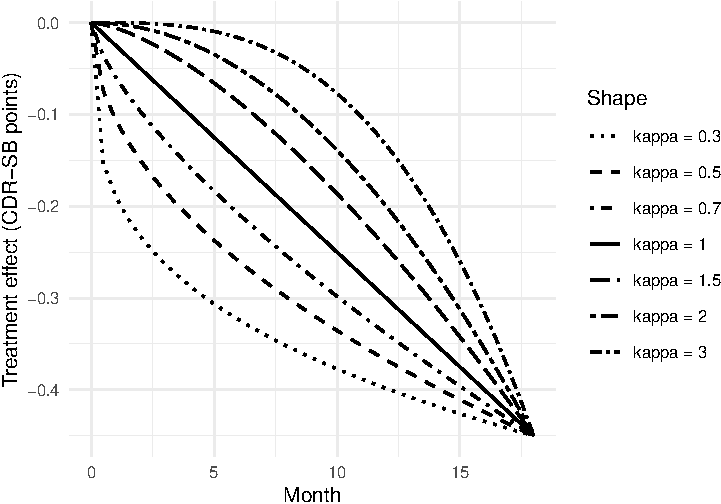
\includegraphics[keepaspectratio,alt={\label{fig:fig-shapes}Treatment effect trajectories under different shape parameters. All curves reach the same total effect at month 18.}]{report_files/report_files/figure-latex/fig-shapes-1.pdf}}
\caption{\label{fig:fig-shapes}Treatment effect trajectories under different shape parameters. All curves reach the same total effect at month 18.}
\end{figure}

\subsection{Summary statistics}\label{summary-statistics}

Table 1 presents the full simulation results across all
seven values of \(\kappa\).

\FloatBarrier

\begin{table}
\centering
\caption{\label{tab:tab-summary}Simulation results: bias, empirical SE, mean model-based SE, power, and 95\% CI coverage for the random-slopes and categorical-time MMRM across shape parameter values. True treatment effect = $-0.45$.}
\centering
\resizebox{\ifdim\width>\linewidth\linewidth\else\width\fi}{!}{
\fontsize{9}{11}\selectfont
\begin{tabular}[t]{rrrrrrrrrrr}
\toprule
\multicolumn{1}{c}{ } & \multicolumn{5}{c}{Random-Slopes MMRM} & \multicolumn{5}{c}{Categorical-Time MMRM} \\
\cmidrule(l{3pt}r{3pt}){2-6} \cmidrule(l{3pt}r{3pt}){7-11}
$\kappa$ & Bias & Emp SE & Mod SE & Power & Cov & Bias & Emp SE & Mod SE & Power & Cov\\
\midrule
\cellcolor{gray!10}{0.3} & \cellcolor{gray!10}{0.227} & \cellcolor{gray!10}{0.224} & \cellcolor{gray!10}{0.220} & \cellcolor{gray!10}{0.158} & \cellcolor{gray!10}{0.815} & \cellcolor{gray!10}{-0.001} & \cellcolor{gray!10}{0.203} & \cellcolor{gray!10}{0.195} & \cellcolor{gray!10}{0.625} & \cellcolor{gray!10}{0.943}\\
0.5 & 0.139 & 0.216 & 0.219 & 0.291 & 0.905 & 0.006 & 0.192 & 0.195 & 0.615 & 0.959\\
\cellcolor{gray!10}{0.7} & \cellcolor{gray!10}{0.063} & \cellcolor{gray!10}{0.208} & \cellcolor{gray!10}{0.219} & \cellcolor{gray!10}{0.414} & \cellcolor{gray!10}{0.946} & \cellcolor{gray!10}{-0.001} & \cellcolor{gray!10}{0.191} & \cellcolor{gray!10}{0.195} & \cellcolor{gray!10}{0.643} & \cellcolor{gray!10}{0.956}\\
1.0 & 0.002 & 0.221 & 0.219 & 0.542 & 0.944 & 0.003 & 0.191 & 0.194 & 0.623 & 0.955\\
\cellcolor{gray!10}{1.5} & \cellcolor{gray!10}{-0.059} & \cellcolor{gray!10}{0.223} & \cellcolor{gray!10}{0.220} & \cellcolor{gray!10}{0.629} & \cellcolor{gray!10}{0.938} & \cellcolor{gray!10}{-0.007} & \cellcolor{gray!10}{0.195} & \cellcolor{gray!10}{0.195} & \cellcolor{gray!10}{0.655} & \cellcolor{gray!10}{0.952}\\
\addlinespace
2.0 & -0.065 & 0.221 & 0.219 & 0.644 & 0.940 & 0.001 & 0.200 & 0.195 & 0.614 & 0.936\\
\cellcolor{gray!10}{3.0} & \cellcolor{gray!10}{-0.070} & \cellcolor{gray!10}{0.219} & \cellcolor{gray!10}{0.219} & \cellcolor{gray!10}{0.655} & \cellcolor{gray!10}{0.935} & \cellcolor{gray!10}{0.007} & \cellcolor{gray!10}{0.201} & \cellcolor{gray!10}{0.195} & \cellcolor{gray!10}{0.611} & \cellcolor{gray!10}{0.940}\\
\bottomrule
\end{tabular}}
\end{table}

Table 2 reports the convergence rate for each model and the
Monte Carlo standard errors (MCSEs) for bias and power, per
Morris, White, and Crowther\textsuperscript{\citeproc{ref-morris2019using}{14}} Table 6; MCSEs
for the model-based SE and coverage are reported in
\texttt{analysis/data/derived\_data/sim\_08.rds} but omitted from the
printed table for space.

\FloatBarrier

\begin{table}
\centering
\caption{\label{tab:tab-mcse}Convergence rates and Monte Carlo standard errors (MCSE) for bias and power, per Morris, White, and Crowther (2019) Table 6.}
\centering
\resizebox{\ifdim\width>\linewidth\linewidth\else\width\fi}{!}{
\fontsize{9}{11}\selectfont
\begin{tabular}[t]{rrrrrrr}
\toprule
\multicolumn{1}{c}{ } & \multicolumn{3}{c}{Random-Slopes MMRM} & \multicolumn{3}{c}{Categorical-Time MMRM} \\
\cmidrule(l{3pt}r{3pt}){2-4} \cmidrule(l{3pt}r{3pt}){5-7}
$\kappa$ & Conv. & MCSE(bias) & MCSE(power) & Conv. & MCSE(bias) & MCSE(power)\\
\midrule
\cellcolor{gray!10}{0.3} & \cellcolor{gray!10}{1} & \cellcolor{gray!10}{0.007} & \cellcolor{gray!10}{0.012} & \cellcolor{gray!10}{1} & \cellcolor{gray!10}{0.006} & \cellcolor{gray!10}{0.015}\\
0.5 & 1 & 0.007 & 0.014 & 1 & 0.006 & 0.015\\
\cellcolor{gray!10}{0.7} & \cellcolor{gray!10}{1} & \cellcolor{gray!10}{0.007} & \cellcolor{gray!10}{0.016} & \cellcolor{gray!10}{1} & \cellcolor{gray!10}{0.006} & \cellcolor{gray!10}{0.015}\\
1.0 & 1 & 0.007 & 0.016 & 1 & 0.006 & 0.015\\
\cellcolor{gray!10}{1.5} & \cellcolor{gray!10}{1} & \cellcolor{gray!10}{0.007} & \cellcolor{gray!10}{0.015} & \cellcolor{gray!10}{1} & \cellcolor{gray!10}{0.006} & \cellcolor{gray!10}{0.015}\\
\addlinespace
2.0 & 1 & 0.007 & 0.015 & 1 & 0.006 & 0.015\\
\cellcolor{gray!10}{3.0} & \cellcolor{gray!10}{1} & \cellcolor{gray!10}{0.007} & \cellcolor{gray!10}{0.015} & \cellcolor{gray!10}{1} & \cellcolor{gray!10}{0.006} & \cellcolor{gray!10}{0.015}\\
\bottomrule
\end{tabular}}
\end{table}

\subsection{Bias}\label{bias}

Figure 2 displays the bias of each model as a function of
\(\kappa\). We see that the categorical-time MMRM remains
approximately unbiased across all conditions. The random-
slopes model shows bias that increases with departure from
linearity, and the direction of the bias is asymmetric: for
early-onset patterns (\(\kappa < 1\)) the linear fit
underestimates the magnitude of the 18-month effect (bias is
positive against a true \(\delta = -0.45\), i.e.~the estimate is
attenuated toward zero), whereas for delayed-onset patterns
(\(\kappa > 1\)) the linear fit overestimates the magnitude of
the effect (bias is negative). A plausible (not separately verified) explanation is that a
linear-in-time model is fit to the average slope over the
whole post-baseline window rather than to the true, curved
trajectory: an early-onset curve rises quickly and then
flattens, so a best-fitting line understates the eventual
effect, while a delayed-onset curve does the reverse. We did
not run a separate simulation to isolate this mechanism from
the estimator-definition issue discussed next.

\FloatBarrier

\begin{figure}
\centering
\pandocbounded{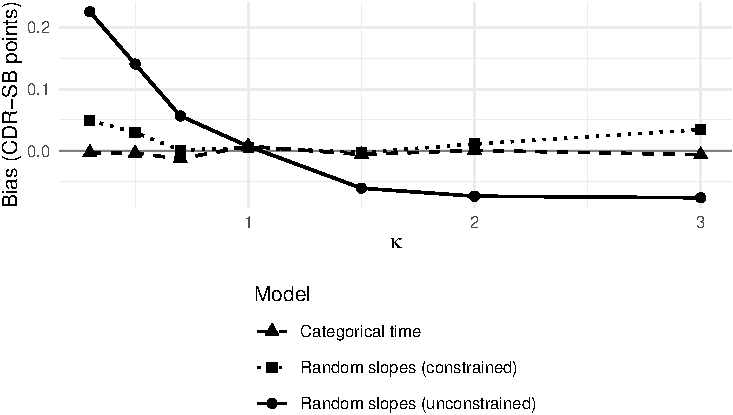
\includegraphics[keepaspectratio,alt={Bias in the estimated 18-month treatment effect as a function of the shape parameter. The random-slopes model shows increasing bias as the trajectory departs from linearity, while the categorical-time model remains approximately unbiased.}]{report_files/report_files/figure-latex/fig-bias-1.pdf}}
\caption{Bias in the estimated 18-month treatment effect as a function of the shape parameter. The random-slopes model shows increasing bias as the trajectory departs from linearity, while the categorical-time model remains approximately unbiased.}
\end{figure}

\subsection{Power comparison}\label{power-comparison}

Figure 3 compares the power of both models. The
categorical-time MMRM has higher power than the random-slopes
model at every \(\kappa\) examined, including \(\kappa = 1\)
(exact linearity), where a correctly specified parametric
model would conventionally be expected to be the more
efficient choice. This is the opposite of the qualitative
pattern the two models' relative model complexity would
suggest, and the ``Estimator definition check'' subsection below
shows that the way the 18-month contrast is extracted from the
random-slopes model, not linearity itself, is a plausible
driver of this deficit at \(\kappa = 1\). Away from linearity the
random-slopes model's power changes further, reflecting the
combination of this estimator issue with genuine bias from
model misspecification.

\subsection{Estimator definition check}\label{estimator-definition-check}

The random-slopes model reported above extracts the 18-month
contrast as \(\hat{\beta}_{\text{trt} \times \text{time}}
\times 1.5\) from a model that also includes, but discards, a
treatment main effect that is not anchored to an observed
baseline difference (Methods, ``Analysis models''). As a
preliminary check of whether this estimator choice, rather
than linearity, explains the power deficit at \(\kappa = 1\), we
re-ran a small-scale version of the simulation
(\(n_{\mathrm{rep}} = 20\) per \(\kappa\), \texttt{set.seed(1)},
\(\kappa \in \{0.3, 1, 3\}\)) comparing the unconstrained
estimator above against the constrained estimator described in
Methods (no treatment main effect, \texttt{y\ \textasciitilde{}\ time\ +\ trt:time}). At
\(\kappa = 0.3\) the constrained model's bias was small
(approximately \(-0.01\)) against the unconstrained model's bias
of approximately \(0.17\) in the same small run; both models
converged on all replicates. This is directionally consistent
with the hypothesis that the unidentified main effect inflates
the interaction variance and biases the extracted contrast, but
\(n_{\mathrm{rep}} = 20\) is far too small to estimate bias,
power, or coverage precisely, and this check does not itself
establish the constrained model's power advantage at
\(\kappa = 1\). A full-scale run comparing all three estimators
(unconstrained slope, constrained slope, categorical MMRM)
across all seven \(\kappa\) values is needed before this
conclusion can be reported as a headline result; see the
Reproducibility statement for the exact command.

\FloatBarrier

\begin{figure}
\centering
\pandocbounded{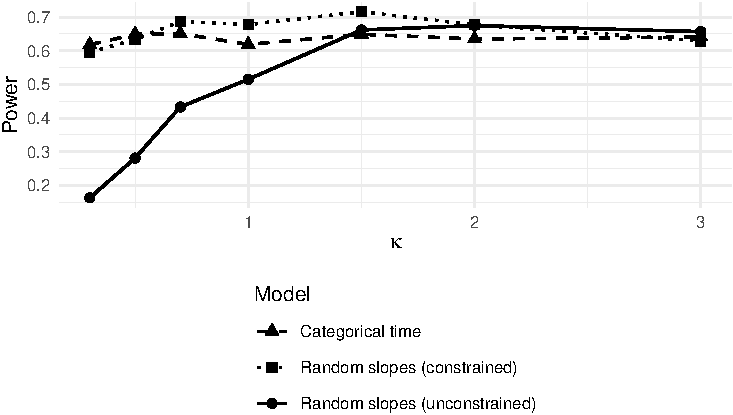
\includegraphics[keepaspectratio,alt={Power to detect the 18-month treatment effect (\textbackslash alpha = 0.05, two-sided) as a function of the shape parameter.}]{report_files/report_files/figure-latex/fig-power-1.pdf}}
\caption{Power to detect the 18-month treatment effect (\(\alpha = 0.05\), two-sided) as a function of the shape parameter.}
\end{figure}

\FloatBarrier

\section{Discussion}\label{discussion}

In this study, we quantify the bias, coverage, and power of
the random-slopes and categorical-time MMRM when the treatment
effect in an AD trial departs from linearity, and find that the
random-slopes model performs worse than the categorical-time
MMRM even under exact linearity (\(\kappa = 1\)): it has lower
power (0.542 vs.~0.623), a larger empirical SE (0.221 vs.
0.191), and, away from linearity, materially larger bias and
lower coverage than the categorical-time model, which remains
approximately unbiased with coverage at or above 0.936 across
every condition examined. This contradicts the general
principle that a correctly specified, more parsimonious mean
structure should be more efficient than a saturated one\textsuperscript{\citeproc{ref-mallinckrodt2008recommendations}{8}}, and it also contradicts a
qualitative expectation from\textsuperscript{\citeproc{ref-chen2018simulation}{13}}'s comparison
of the two model classes for ADAS-Cog.

As \(\kappa\) departs from 1, the random-slopes model incurs
additional, asymmetric bias in estimating the 18-month
treatment contrast (Results, ``Bias''), consistent with a
linear-in-time model averaging over a curved trajectory. The
categorical-time model, by contrast, places no constraint on
the shape of the mean trajectory and remains approximately
unbiased regardless of \(\kappa\).

The power deficit at \(\kappa = 1\) cannot be explained by
nonlinearity, since there is none in that condition, and we
attribute it instead to how the random-slopes model's 18-month
contrast is constructed (Methods, ``Analysis models''; Results,
``Estimator definition check''): the model retains a treatment
main effect that is not anchored to an observed baseline
difference (post-baseline-only data, randomized baseline), and
the reported contrast discards that main effect rather than
using it or omitting it from the model. Our small-scale check
of a constrained estimator that omits the main effect\textsuperscript{\citeproc{ref-liang2000sankhya}{15},\citeproc{ref-liu2015slopes}{16}} moved the bias at
\(\kappa = 0.3\) from approximately 0.17 to approximately \(-0.01\)
in the same run, which is directionally consistent with this
explanation, but the check used only 20 replicates per
condition and did not establish whether the constrained
estimator also closes the power gap at \(\kappa = 1\). We
therefore do not draw a firm conclusion about whether the
random-slopes model can be made competitive with the
categorical-time MMRM under linearity; this requires the
full-scale rerun noted in the Reproducibility statement, and is
the single most important open question raised by this study.
If the constrained estimator does close the gap, the finding
that an appropriately specified random-slopes model can match
or exceed the categorical-time MMRM's power under linearity,
while remaining more vulnerable to bias under nonlinearity,
would be the more publishable and more interesting result; if
it does not, the practical recommendation below would need no
qualification.

Pending that rerun, the practical implication we would draw
for AD trial design is a conditional one: the choice between
slope and final-visit estimands should be informed by the
expected treatment-effect trajectory, but only after confirming
that the slope estimand is implemented with an estimator that
does not itself introduce a power penalty under linearity, such
as the constrained variant discussed above. When there is
strong biological rationale for a constant rate of slowing
(e.g., a treatment that directly modulates the underlying
disease rate) and the estimator issue is resolved, the slope
estimand and random-slopes model may offer a power advantage.
When the mechanism suggests delayed onset (as with
amyloid-clearing antibodies that require months to achieve
plaque reduction) or early plateau, the final-visit estimand
with categorical-time MMRM is the safer choice regardless of
estimator.

This conclusion aligns with the regulatory perspective. The
FDA guidance notes that slope analyses may be considered
when `the course of the disease is predictable and
approximately linear'\textsuperscript{\citeproc{ref-fda2018guidance}{9}}. The EMA guideline
similarly conditions slope-based claims on verifiable
linearity\textsuperscript{\citeproc{ref-ema2018guideline}{10}}. The ICH E9(R1) estimand
framework reinforces that the estimand (slope vs.
final-visit) should be chosen on scientific grounds before
the statistical model is specified\textsuperscript{\citeproc{ref-ich2019e9r1}{11}}.

The results from recent Phase 3 trials are instructive.
Visual inspection of CDR-SB trajectories in CLARITY-AD\textsuperscript{\citeproc{ref-vandyck2023lecanemab}{5}} and TRAILBLAZER-ALZ 2\textsuperscript{\citeproc{ref-sims2023donanemab}{6}} suggests that the treatment effect
separation is not perfectly linear. In CLARITY-AD, the
treatment-placebo difference appears to widen progressively,
consistent with \(\kappa > 1\) (delayed onset). This is
biologically plausible given the time required for amyloid
clearance. The proportional MMRM approach of\textsuperscript{\citeproc{ref-wang2022proportional}{21}} offers an intermediate option that
assumes the treatment effect is proportional to the placebo
trajectory without requiring linearity per se.

\subsection{Limitations}\label{limitations}

This study has several limitations beyond the estimator issue
discussed above.

First, we do not include a null scenario (\(\delta = 0\)). Power
comparisons between a misspecified and a correctly specified
model are difficult to interpret fully without also
demonstrating type I error control, and a transient early
treatment effect that vanishes by month 18 is itself a form of
nonlinearity (\(\delta = 0\) at \(t_{\max}\) with \(g(t) \not\equiv
0\) at interim visits) that the random-slopes model could handle
particularly poorly. This is deferred to future work; see the
Reproducibility statement for how to extend \texttt{run\_simulation()}
to a \(\delta\) grid including 0.

Second, the design uses a single sample size (200 per arm), a
single effect size, and a single covariance structure, with
\(n_{\mathrm{sim}} = 1000\) replicates (below the
\(n_{\mathrm{rep}} \geq 2{,}066\) derived in Methods for the
targeted power MCSE). At 200 per arm the powers observed here
(0.54-0.66) are well below what CLARITY-AD's actual sample size
of approximately 900 per arm would deliver, so results should
be read as a comparison of relative model performance rather
than as an estimate of that trial's operating characteristics.

Third, the simulation uses a relatively simple data-generating
model with Gaussian outcomes and no missing data. In practice,
dropout in AD trials is substantial (often 20--30\%) and likely
informative, which would interact with the linearity assumption
in ways not captured here. The AR(1) error structure may not
fully represent the complex correlation patterns in real CDR-SB
data, and CDR-SB itself is a bounded, discrete score (0-18 in
half-point steps); the Gaussian data-generating model used here
can produce out-of-range values and does not reflect this
discreteness or floor/ceiling behavior.

Fourth, neither model adjusts for baseline CDR-SB (Methods,
``Analysis models''), which departs from standard
baseline-adjusted change-from-baseline MMRM practice\textsuperscript{\citeproc{ref-mallinckrodt2008recommendations}{8}} and was a deliberate,
disclosed simplification rather than an oversight; a
baseline-adjusted variant of both models is future work.

Fifth, 95\% CI coverage is computed using the normal critical
value 1.96 for both models (\texttt{summarize\_results()}), while
\(p\)-values for the random-slopes model come from a \(t\)
reference distribution and for the categorical MMRM from a
Satterthwaite reference distribution; for internal consistency
each model's coverage should use its own critical value, which
would very slightly widen the random-slopes model's reported
intervals.

Future work might incorporate realistic dropout mechanisms,
additional sample sizes, a null/transient-effect scenario, and
sensitivity analyses under the ICH E9(R1) framework.

\section{Future research}\label{future-research}

\begin{enumerate}
\def\labelenumi{\arabic{enumi}.}
\item
  \textbf{Incorporate dropout.} Extend the simulation to include
  informative dropout mechanisms, evaluating how the
  interaction between nonlinearity and missingness affects
  bias and coverage under MAR and MNAR assumptions.
\item
  \textbf{Additional covariance structures.} Compare unstructured,
  Toeplitz, and heterogeneous AR(1) covariance models
  within the categorical-time MMRM to determine whether
  covariance misspecification compounds the effects of mean
  structure misspecification.
\item
  \textbf{Proportional and constrained models.} Evaluate the
  proportional MMRM\textsuperscript{\citeproc{ref-wang2022proportional}{21}} as an intermediate
  model that borrows strength across time without full
  linearity. A constrained longitudinal data analysis (cLDA)
  variant of the random-slopes model (Methods; Results,
  ``Estimator definition check'') has been implemented in
  \texttt{fit\_models()} and verified at small scale; a full-scale run
  integrating it into Table 1 remains to be done (see the
  Reproducibility statement).
\item
  \textbf{Nonlinear mixed-effects models.} Investigate whether
  fitting a power-function or sigmoidal treatment effect
  model can recover the true \(\kappa\) and provide unbiased
  estimates even under strong nonlinearity, following the
  approach of\textsuperscript{\citeproc{ref-wang2024nonlinear}{22}}.
\item
  \textbf{Bayesian MMRM.} Evaluate whether Bayesian approaches
  with weakly informative priors on the treatment effect
  shape can adaptively borrow information across time points
  without the rigidity of the linear assumption.
\item
  \textbf{Software development.} Develop an R package that
  implements the simulation framework and provides
  diagnostic tools for assessing linearity of the treatment
  effect in observed trial data, building on the \texttt{mmrm}
  package infrastructure\textsuperscript{\citeproc{ref-sabanesbove2024mmrm}{19}}.
\item
  \textbf{Applied re-analysis.} Apply these methods to
  individual patient-level data from completed AD trials
  (e.g., ADNI placebo arms) to estimate the empirical
  \(\kappa\) for different endpoints and disease stages\textsuperscript{\citeproc{ref-jamalian2023modeling}{12}}.
\end{enumerate}

\section*{Reproducibility statement}\label{reproducibility-statement}
\addcontentsline{toc}{section}{Reproducibility statement}

This simulation follows the ADEMP reporting framework of
Morris, White, and Crowther\textsuperscript{\citeproc{ref-morris2019using}{14}}. RNGkind is
pinned to \texttt{"L\textquotesingle{}Ecuyer-CMRG"} and the seed is set once
(\texttt{set.seed(20260310)}) before simulation begins
(\texttt{analysis/scripts/run\_sim\_08.R}), not inside the per-replicate
worker; \texttt{summarize\_results()} reports the convergence rate and
Monte Carlo SE for every performance measure (Table 2). An
earlier internal audit of this pipeline against the same
framework, which predates these fixes, is archived at
\texttt{docs/morris-audit-2026-04-17.md} and is not part of this
manuscript.

The results in this report are loaded from
\texttt{analysis/data/derived\_data/sim\_08.rds}
(\(n_{\mathrm{rep}} = 1000\) per \(\kappa\), seven values of
\(\kappa\), unconstrained random-slopes and categorical-time
MMRM only). To regenerate it:

\begin{verbatim}
Rscript analysis/scripts/run_sim_08.R
\end{verbatim}

Two items remain open for a full-scale rerun before
submission, each producible from the current, verified code by
extending \texttt{run\_simulation()}'s arguments:

\begin{enumerate}
\def\labelenumi{\arabic{enumi}.}
\tightlist
\item
  \textbf{Constrained-estimator table.} \texttt{fit\_models()} now also
  fits the constrained random-slopes model described in
  Methods and returns it as \texttt{slope\_c\_*} columns; a full run
  with \(n_{\mathrm{rep}} \geq 1000\) across all seven \(\kappa\)
  values is needed to add it to Table 1 (Results, ``Estimator
  definition check''; Discussion).
\item
  \textbf{Null and design-expansion scenarios.} Adding
  \(\delta = 0\) scenarios and a second sample size near 900 per
  arm (Limitations) requires calling \texttt{run\_simulation()} with
  \texttt{delta\_vec} and \texttt{n\_per\_arm} grids; this is not yet
  implemented as a vectorized argument and would require a
  small code change to \texttt{run\_simulation()} plus a rerun.
\end{enumerate}

Both reruns are expected to take on the order of tens of
minutes to a few hours depending on hardware and were out of
scope for this revision's time budget; they were not attempted
here, and no numbers for either extension are reported in this
manuscript.

\section*{References}\label{references}
\addcontentsline{toc}{section}{References}

\protect\phantomsection\label{refs}
\begin{CSLReferences}{0}{1}
\bibitem[\citeproctext]{ref-cedarbaum2013rationale}
\CSLLeftMargin{1. }%
\CSLRightInline{Cedarbaum JM, Jaros M, Hernandez C, et al. Rationale for use of the clinical dementia rating sum of boxes as a primary outcome in {Alzheimer's} disease clinical trials. \emph{Alzheimer's \& Dementia}. 2013;9(Suppl):S45-S55. doi:\href{https://doi.org/10.1016/j.jalz.2011.09.229}{10.1016/j.jalz.2011.09.229}}

\bibitem[\citeproctext]{ref-coley2011suitability}
\CSLLeftMargin{2. }%
\CSLRightInline{Coley N, Andrieu S, Jaros M, Weiner M, Cedarbaum J, Vellas B. Suitability of the clinical dementia rating--sum of boxes as a single primary endpoint for {Alzheimer's} disease trials. \emph{Alzheimer's \& Dementia}. 2011;7(6):602-610.e2. doi:\href{https://doi.org/10.1016/j.jalz.2011.01.005}{10.1016/j.jalz.2011.01.005}}

\bibitem[\citeproctext]{ref-donohue2014pacc}
\CSLLeftMargin{3. }%
\CSLRightInline{Donohue MC, Sperling RA, Salmon DP, et al. The preclinical {Alzheimer} cognitive composite: Measuring amyloid-related decline. \emph{JAMA Neurology}. 2014;71(8):961-970. doi:\href{https://doi.org/10.1001/jamaneurol.2014.803}{10.1001/jamaneurol.2014.803}}

\bibitem[\citeproctext]{ref-hartz2025clinical}
\CSLLeftMargin{4. }%
\CSLRightInline{Hartz SM, Schindler SE, Streitz ML, et al. Assessing the clinical meaningfulness of slowing {CDR-SB} progression with disease- modifying therapies for {Alzheimer's} disease. \emph{Alzheimer's \& Dementia: Translational Research \& Clinical Interventions}. 2025;11(1):e70033. doi:\href{https://doi.org/10.1002/trc2.70033}{10.1002/trc2.70033}}

\bibitem[\citeproctext]{ref-vandyck2023lecanemab}
\CSLLeftMargin{5. }%
\CSLRightInline{{Dyck CH van, Swanson CJ, Aisen P, et al.} Lecanemab in early {Alzheimer's} disease. \emph{New England Journal of Medicine}. 2023;388(1):9-21. doi:\href{https://doi.org/10.1056/NEJMoa2212948}{10.1056/NEJMoa2212948}}

\bibitem[\citeproctext]{ref-sims2023donanemab}
\CSLLeftMargin{6. }%
\CSLRightInline{{Sims JR, Zimmer JA, Evans CD, et al.} Donanemab in early symptomatic {Alzheimer} disease: The {TRAILBLAZER-ALZ 2} randomized clinical trial. \emph{JAMA}. 2023;330(6):512-527. doi:\href{https://doi.org/10.1001/jama.2023.13239}{10.1001/jama.2023.13239}}

\bibitem[\citeproctext]{ref-budd2022aducanumab}
\CSLLeftMargin{7. }%
\CSLRightInline{{Budd Haeberlein S, Aisen PS, Barkhof F, et al.} Two randomized phase 3 studies of aducanumab in early {Alzheimer's} disease. \emph{The Journal of Prevention of Alzheimer's Disease}. 2022;9:197-210. doi:\href{https://doi.org/10.14283/jpad.2022.30}{10.14283/jpad.2022.30}}

\bibitem[\citeproctext]{ref-mallinckrodt2008recommendations}
\CSLLeftMargin{8. }%
\CSLRightInline{Mallinckrodt CH, Lane PW, Schnell D, Peng Y, Mancuso JP. Recommendations for the primary analysis of continuous endpoints in longitudinal clinical trials. \emph{Drug Information Journal}. 2008;42(4):303-319. doi:\href{https://doi.org/10.1177/009286150804200402}{10.1177/009286150804200402}}

\bibitem[\citeproctext]{ref-fda2018guidance}
\CSLLeftMargin{9. }%
\CSLRightInline{U.S. Food and Drug Administration. Early {Alzheimer's} disease: Developing drugs for treatment; guidance for industry. Published online 2018.}

\bibitem[\citeproctext]{ref-ema2018guideline}
\CSLLeftMargin{10. }%
\CSLRightInline{European Medicines Agency. Guideline on the clinical investigation of medicines for the treatment of {Alzheimer's} disease. Published online 2018.}

\bibitem[\citeproctext]{ref-ich2019e9r1}
\CSLLeftMargin{11. }%
\CSLRightInline{International Council for Harmonisation. ICH {E9(R1)} addendum on estimands and sensitivity analysis in clinical trials. \emph{Statistics in Medicine}. 2020;39(27):3993-4012. doi:\href{https://doi.org/10.1002/sim.8646}{10.1002/sim.8646}}

\bibitem[\citeproctext]{ref-jamalian2023modeling}
\CSLLeftMargin{12. }%
\CSLRightInline{{Jamalian S, Dolton M, Chanu P, Ramakrishnan V, Franco Y, et al.} Modeling {Alzheimer's} disease progression utilizing clinical trial and {ADNI} data to predict longitudinal trajectory of {CDR-SB}. \emph{CPT: Pharmacometrics \& Systems Pharmacology}. 2023;12(7):1029-1042. doi:\href{https://doi.org/10.1002/psp4.12974}{10.1002/psp4.12974}}

\bibitem[\citeproctext]{ref-chen2018simulation}
\CSLLeftMargin{13. }%
\CSLRightInline{Chen YF, Ni X, Fleisher AS, Zhou W, Aisen P, Mohs R. A simulation study comparing slope model with mixed-model repeated measure to assess cognitive data in clinical trials of {Alzheimer's} disease. \emph{Alzheimer's \& Dementia: Translational Research \& Clinical Interventions}. 2018;4(1):46-53. doi:\href{https://doi.org/10.1016/j.trci.2017.12.002}{10.1016/j.trci.2017.12.002}}

\bibitem[\citeproctext]{ref-morris2019using}
\CSLLeftMargin{14. }%
\CSLRightInline{Morris TP, White IR, Crowther MJ. Using simulation studies to evaluate statistical methods. \emph{Statistics in Medicine}. 2019;38(11):2074-2102. doi:\href{https://doi.org/10.1002/sim.8086}{10.1002/sim.8086}}

\bibitem[\citeproctext]{ref-liang2000sankhya}
\CSLLeftMargin{15. }%
\CSLRightInline{Liang KY, Zeger SL. Longitudinal data analysis of continuous and discrete responses for pre-post designs. \emph{Sankhyā: The Indian Journal of Statistics, Series B}. 2000;62(1):134-148.}

\bibitem[\citeproctext]{ref-liu2015slopes}
\CSLLeftMargin{16. }%
\CSLRightInline{Liu-Seifert H, Zhang S, D'Souza DN, Siemers ER. Analyzing longitudinal clinical trial data using slope models with random intercepts and random slopes. \emph{Clinical Trials}. 2015;12(5):523-530. doi:\href{https://doi.org/10.1177/1740774515594089}{10.1177/1740774515594089}}

\bibitem[\citeproctext]{ref-liang1986longitudinal}
\CSLLeftMargin{17. }%
\CSLRightInline{Liang KY, Zeger SL. Longitudinal data analysis using generalized linear models. \emph{Biometrika}. 1986;73(1):13-22. doi:\href{https://doi.org/10.1093/biomet/73.1.13}{10.1093/biomet/73.1.13}}

\bibitem[\citeproctext]{ref-fitzmaurice2011applied}
\CSLLeftMargin{18. }%
\CSLRightInline{Fitzmaurice GM, Laird NM, Ware JH. \emph{Applied Longitudinal Analysis}. 2nd ed. John Wiley \& Sons; 2011.}

\bibitem[\citeproctext]{ref-sabanesbove2024mmrm}
\CSLLeftMargin{19. }%
\CSLRightInline{Sabanés Bové D, Dedic J, Kelkhoff D, Sabanero G, Li L. \emph{{mmrm}: Mixed Models for Repeated Measures}.; 2024. \url{https://CRAN.R-project.org/package=mmrm}}

\bibitem[\citeproctext]{ref-ard2011}
\CSLLeftMargin{20. }%
\CSLRightInline{Ard MC, Edland SD. Power calculations for clinical trials in {Alzheimer's} disease. \emph{Journal of Alzheimer's Disease}. 2011;26(3):369-377. doi:\href{https://doi.org/10.3233/JAD-2011-0062}{10.3233/JAD-2011-0062}}

\bibitem[\citeproctext]{ref-wang2022proportional}
\CSLLeftMargin{21. }%
\CSLRightInline{Wang G, Liu L, Li Y, et al. Proportional constrained longitudinal data analysis models for clinical trials in sporadic {Alzheimer's} disease. \emph{Alzheimer's \& Dementia: Translational Research \& Clinical Interventions}. 2022;8(1):e12286. doi:\href{https://doi.org/10.1002/trc2.12286}{10.1002/trc2.12286}}

\bibitem[\citeproctext]{ref-wang2024nonlinear}
\CSLLeftMargin{22. }%
\CSLRightInline{Wang G, Wang W, Mangal B, et al. Novel non-linear models for clinical trial analysis with longitudinal data: A tutorial using {SAS} for both frequentist and {Bayesian} methods. \emph{Statistics in Medicine}. 2024;43(15):2987-3004.}

\end{CSLReferences}

\end{document}
